\section{Исследовательский раздел}

% NOTE:
% Данный раздел содержит описание проведенных экспериментов и их результаты
% Должно быть обязательно указано, какую цель ставил перед собой автор работы при планировании экспериментов
% Какие предположения, гипотезы он надеялся подтвердить и опровергнуть и их помощью
% Результаты оформляются в виде графиков, диаграмм и/или таблиц
% (здесь также может быть проведено качественное и количественное сравнение с аналогами)

В данном разделе будет приведено описание исследования, технические характеристики устройства, на котором выполнялись замеры времени, будет представлены и проанализированы результаты исследования.

Целью данного исследования является определение зависимостей времени выполнения разметки и максимального объема используемой памяти в зависимости от количества процессов, выполняющих разметку.

Предположительно, разметка будет производиться наиболее эффективно в случае, когда количество рабочих процессов совпадает с количеством физических ядер процессора.
Также тип разметки не будет влиять на максимальный объем используемой памяти.

% Рек. Объем - 10-15 страниц

\subsection{Описание исследования}

В листинге \ref{lst:bench} ниже и листингах \ref{lst:mainbench} -- \ref{lst:mbf} приложения А представлен исходный код скриптов, запускаемых для выполнения замеров времени и максимального объема используемой во время разметки памяти.

\begin{lstlisting}[caption={bench.py --- Скрипт для запуска теста производительности}, label={lst:bench}]
import subprocess

PDF_PATH = "/home/rukost/report.pdf"
MARKUP_TYPE = "0"
PAGES = "1-50"

for workers in [1, 2, 4, 8, 16, 32, 64]:
    print(f"\n--- Benchmark with {workers} workers ---")
    result = subprocess.run([
        "python", "main-bench.py",
        PDF_PATH,
        MARKUP_TYPE,
        "-w", str(workers),
        "-p", PAGES
    ], capture_output=True, text=True)
    print(result.stdout)
\end{lstlisting}

\newpage

Для получения данных по разным типам разметок, при запуске скрипта bench.py изменялся параметр MARKUP\_TYPE.

Скрипт запускался десять раз для каждого типа разметки, после чего полученные значения усреднялись.

% Исследовать временные характеристики и затраты памяти предложенного метода

\subsection{Технические характеристики}

Технические характеристики устройства, на котором выполнялись замеры времени, представлены ниже.
\begin{enumerate}
    \item Процессор: \texttt{AMD Ryzen 7 4700U} 2.0 ГГц~\cite{amd}, 8 физических ядер, 8 потоков;
    \item Оперативная память: 8 ГБ, \texttt{DDR4}, 3200 МГц;
    \item Операционная система: \texttt{Arch}~\cite{arch};
    \item Версия ядра: \texttt{6.14.9}.
\end{enumerate}

При выполнении замеров времени ноутбук был подключен к сети электропитания, был запущен терминал Alacritty~\cite{alacritty}, в котором выполнялся тест производительности.

\subsection{Результаты исследования}

В данном подразделе будут приведены и проанализированы результаты исследования времени выполнения и максимального объема памяти, затрачиваемой в процессе построчной, первичной, уточненной и объединенной разметок.

\newpage

\subsubsection{Исследование времени выполнения}

В таблице \ref{tab:tama} и на рисунке \ref{fig:tama} представлены полученные в ходе исследования данные.
Данные, приведенные в таблице являются усредненными значениями из десяти замеров.

\begin{table}[H]
    \centering
    \caption{Время выполнения разметки в зависимости от ее типа и количества процессов, с}
    \label{tab:tama}
    \begin{tabular}{|c|c|c|c|c|}
        \hline
        \textbf{Кол-во процессов} & \textbf{Построчн.} & \textbf{Первичн.} & \textbf{Уточн.} & \textbf{Объед.} \\ \hline
        1 & 31.80 & 41.21 & 41.29 & 41.31 \\ \hline
        2 & 16.70 & 21.72 & 21.96 & 22.03 \\ \hline
        4 & 10.16 & 13.05 & 13.11 & 13.19 \\ \hline
        8 & 7.03 & 8.71 & 8.72 & 8.96 \\ \hline
        16 & 7.29 & 8.83 & 8.96 & 9.23 \\ \hline
        32 & 7.40 & 9.23 & 9.24 & 9.47 \\ \hline
        64 & 7.82 & 9.67 & 9.73 & 9.79 \\ \hline
    \end{tabular}
\end{table}

\begin{figure}[H]
	\centering
	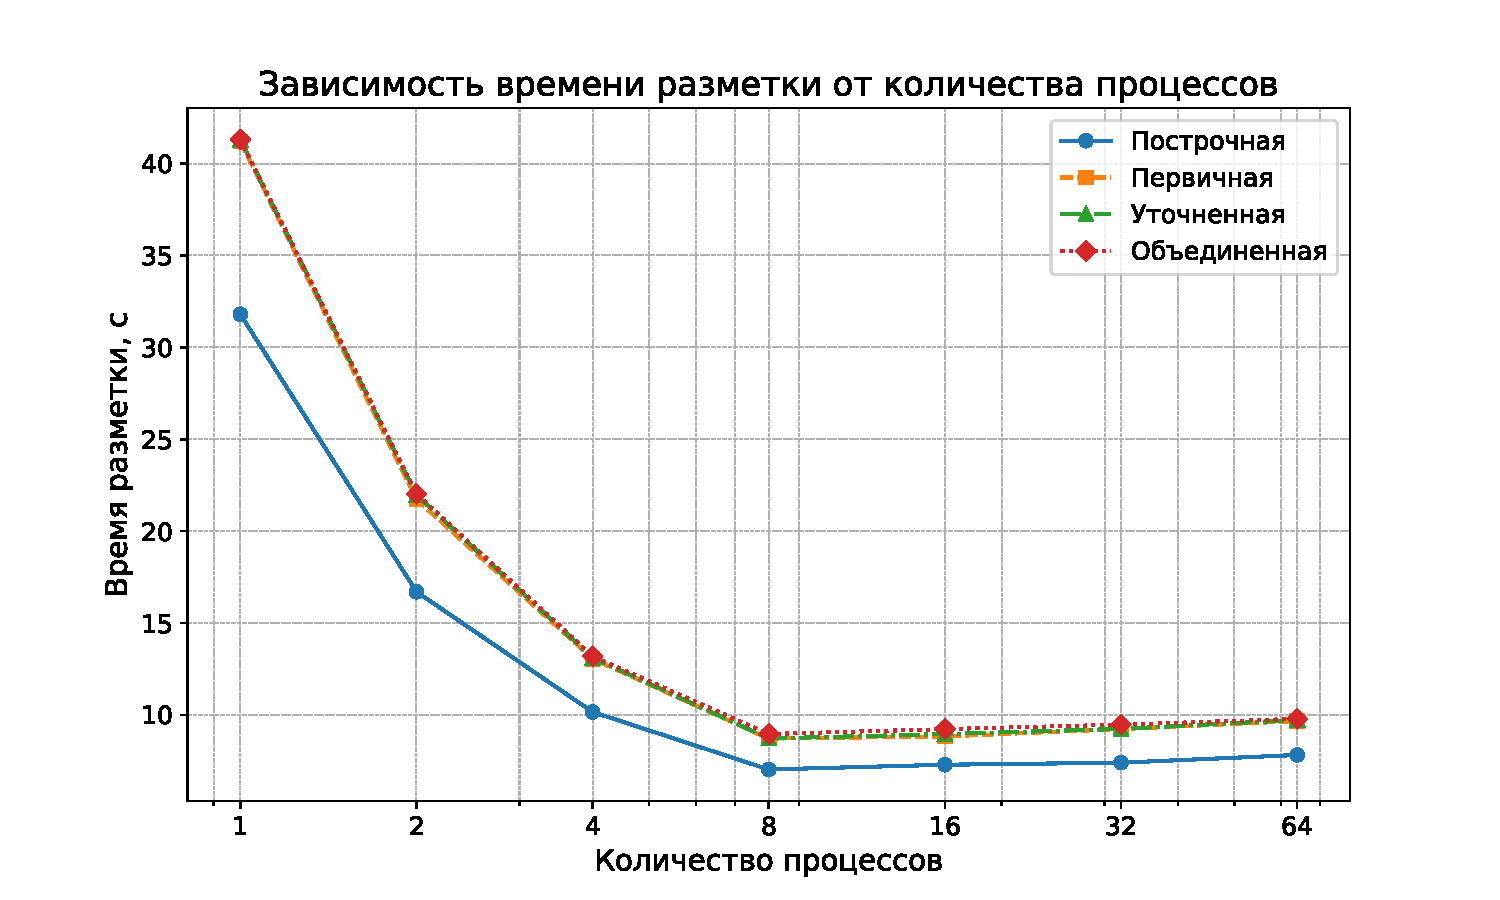
\includegraphics[width=\textwidth]{diag/tama.pdf}
    \caption{Время выполнения разметки в зависимости от ее типа и количества процессов}
	\label{fig:tama}
\end{figure}

\newpage

По полученным данным можно сделать следующие выводы:
\begin{itemize}
    \item Среди разметок наиболее быстрой является построчная, так как для нее нужно меньше вычислений;
    \item Увеличение числа процессов, используемых для разметки, позволяет ускорить процесс разметки;
    \item Наибольшая скорость разметки наблюдается, когда число процессов соответствует числу физических ядер процессора.
\end{itemize}

\subsubsection{Исследование затрачиваемой памяти}

В таблице \ref{tab:pama} и на рисунке \ref{fig:pama} представлены полученные в ходе исследования данные.
Данные, приведенные в таблице являются усредненными значениями из десяти замеров.

\begin{table}[H]
    \centering
    \caption{Максимальное количество памяти, используемое в ходе разметки в зависимости от ее типа и количества процессов, МБ}
    \label{tab:pama}
    \begin{tabular}{|c|c|c|c|c|}
        \hline
        \textbf{Кол-во процессов} & \textbf{Построчн.} & \textbf{Первичн.} & \textbf{Уточн.} & \textbf{Объед.} \\ \hline
        1 & 247.39 & 246.58 & 246.56 & 245.09 \\ \hline
        2 & 374.05 & 373.12 & 373.26 & 373.16 \\ \hline
        4 & 627.94 & 625.74 & 627.79 & 627.11 \\ \hline
        8 & 1085.41 & 1096.95 & 1098.18 & 1122.85 \\ \hline
        16 & 1933.34 & 1934.43 & 1932.78 & 1935.12 \\ \hline
        32 & 3757.83 & 3760.95 & 3758.53 & 3758.38 \\ \hline
        64 & 6437.75 & 6444.76 & 6438.00 & 6440.77 \\ \hline
    \end{tabular}
\end{table}

\begin{figure}[H]
	\centering
	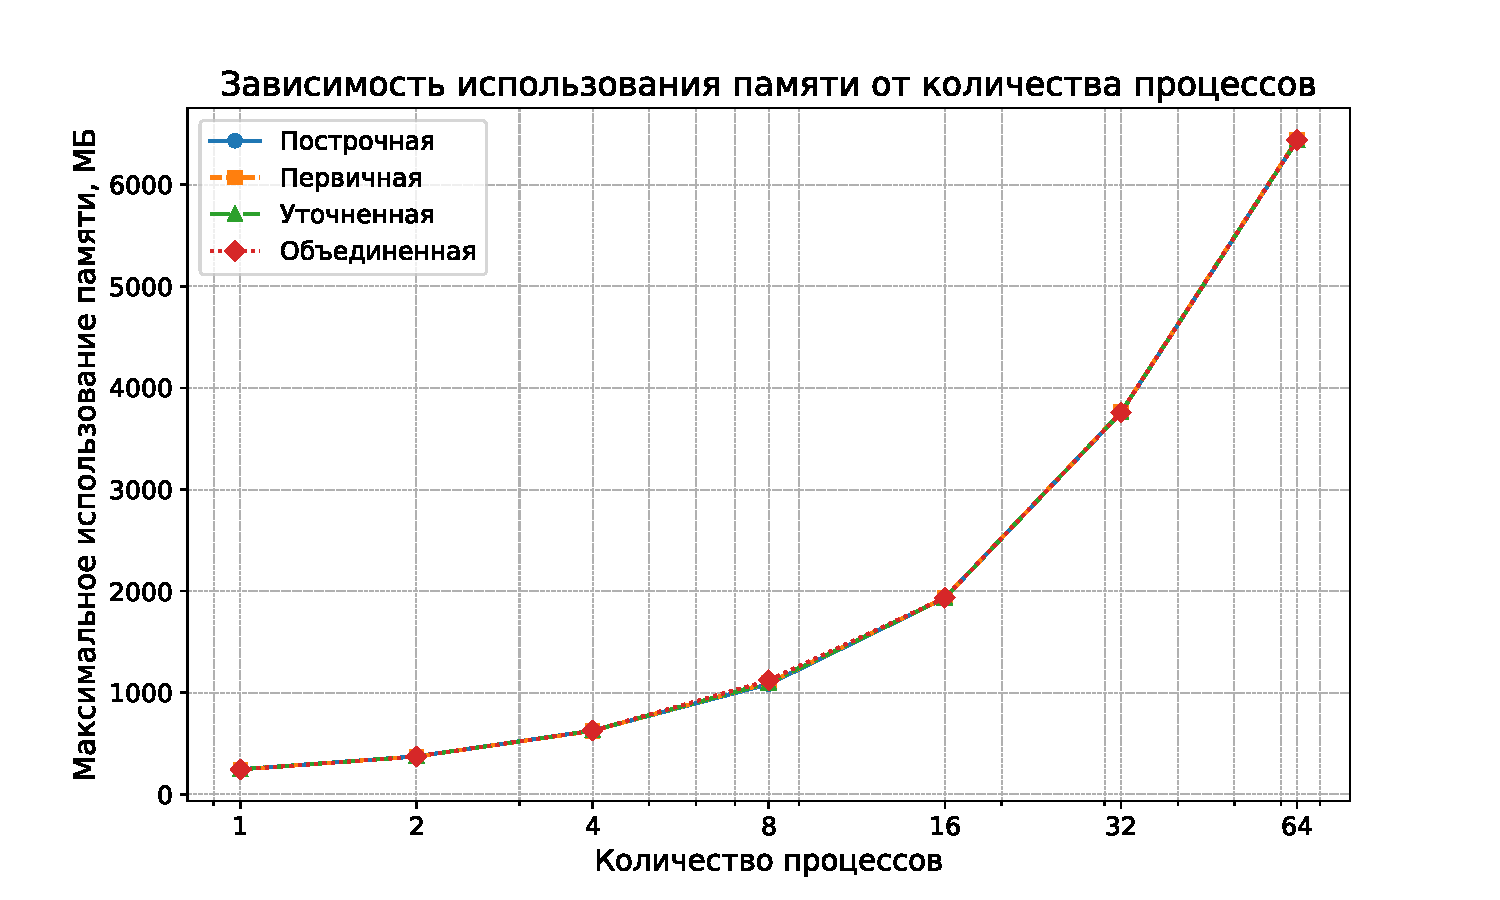
\includegraphics[width=\textwidth]{diag/pama.pdf}
    \caption{Максимальное количество памяти, используемое в ходе разметки в зависимости от ее типа и количества процессов}
	\label{fig:pama}
\end{figure}

По полученным данным можно сделать следующие выводы:
\begin{itemize}
    \item Максимальное количество памяти, используемое при разметке, не зависит от типа разметки;
    \item Основным фактором, влияющим на максимальное количество памяти, используемое при разметке, является количество создаваемых в ходе разметки процессов;
    \item Объем используемой памяти увеличивается прямо пропорционально количеству рабочих процессов.
\end{itemize}

\subsection*{Вывод}

Таким образом, в ходе исследования было выявлено, что разметка наиболее эффективна по времени, когда количество рабочих процессов соответствует количеству физических ядер процессора; самой быстрой является построчная разметка, и объем используемой памяти увеличивается пропорционально количеству рабочих процессов.
